\documentclass[aspectratio=43,10pt]{beamer}

\usecolortheme{seahorse}

\usepackage[T1]{fontenc}
\usepackage[utf8]{inputenc}
\usepackage{lmodern}
\usepackage{zi4}
\usepackage{amsmath,amssymb}
\usepackage{booktabs}
\usepackage{xcolor}
\usepackage{tikz}
\usepackage{listings}

\usetikzlibrary{arrows.meta,positioning,shapes.geometric,calc}

% Colors
\definecolor{AggieMaroon}{HTML}{500000}
\definecolor{CodeBackground}{HTML}{F3F3F3}
\definecolor{CodeBorder}{HTML}{BFBFBF}
\definecolor{CodeComment}{HTML}{666666}
\definecolor{CodeKeyword}{HTML}{2F5597}
\definecolor{Accent}{RGB}{31,78,121}
\definecolor{Good}{RGB}{46,125,50}
\definecolor{Warn}{RGB}{183,91,0}

% Beamer style
\setbeamercolor{structure}{fg=AggieMaroon}
\setbeamertemplate{navigation symbols}{}
\setbeamertemplate{caption}[numbered]

% Blocks
\setbeamercolor{block title}{
  fg=white,
  bg=AggieMaroon
}

\setbeamercolor{block body}{
  fg=black,
  bg=AggieMaroon!8
}

% Alert blocks
\setbeamercolor{block title alerted}{
  fg=white,
  bg=red!70!black
}

\setbeamercolor{block body alerted}{
  fg=black,
  bg=red!8
}

% Rounded blocks
\setbeamertemplate{blocks}[rounded][shadow=false]
\setbeamertemplate{itemize item}{\textbullet}
\setbeamertemplate{itemize subitem}{\textbullet}
\setbeamertemplate{itemize subsubitem}{\textbullet}

\setbeamertemplate{footline}{%
  \hfill
  \textcolor{AggieMaroon}{\insertframenumber/\inserttotalframenumber}
  \hspace{4pt}\vskip2pt
}

% Code style
\lstdefinestyle{classcode}{
  basicstyle=\ttfamily\footnotesize,
  backgroundcolor=\color{CodeBackground},
  frame=single,
  rulecolor=\color{CodeBorder},
  keywordstyle=\color{CodeKeyword}\bfseries,
  commentstyle=\color{CodeComment},
  stringstyle=\color{teal},
  showstringspaces=false,
  keepspaces=true,
  columns=fullflexible,
  breaklines=true,
  tabsize=4
}

% Pseudocode style
\lstdefinestyle{pseudo}{
  basicstyle=\ttfamily\small,
  backgroundcolor=\color{CodeBackground},
  frame=single,
  rulecolor=\color{CodeBorder},
  columns=fullflexible,
  keepspaces=true,
  showstringspaces=false,
  keywordstyle=\bfseries\color{Accent},
  commentstyle=\itshape\color{Good},
  morekeywords={
    Algorithm,Input,Output,for,while,if,else,return,
    then,to,do,not,and,or,true,false
  }
}

\AtBeginSection[]{
  \begin{frame}
    \centering
    \Huge \insertsection
  \end{frame}
}

\lstset{style=classcode}

% Title
\title{1. Python and Jupyter}
\subtitle{Functions, Debugging, and Profiling}
\author{}

\date{%
  \textcolor{AggieMaroon}{
    DAEN 300\\
    \textbf{Alexander Abuabara}\\
    Fall 2026
  }
}

\titlegraphic{
  
\includegraphics[height=1.2cm]{TAMU_logo.png}
}

\begin{document}

%------------------------------------------------
\begin{frame}
  \titlepage
\end{frame}

%------------------------------------------------
\begin{frame}{Goal for Today}

\begin{itemize}
  \item 
  \item Define and use Python functions.
  \item Use Jupyter/IPython tools to investigate errors.
  \item Read and interpret Python tracebacks.
  \item Measure execution time using \texttt{\%time} and \texttt{\%timeit}.
  \item Use profiling tools to identify performance bottlenecks.
\end{itemize}

\end{frame}

%------------------------------------------------
\begin{frame}{Goal for Semester}
\large

\begin{quote}
Let us change our traditional attitude to the construction of programs.
Instead of imagining that our main task is to instruct a computer what to to,
let us concentrate rather on explaining to human beings what we want a computer to do.
\end{quote}

\hfill 
\href{https://en.wikipedia.org/wiki/Donald_Knuth}{Donald Knuth}, 
\href{https://en.wikipedia.org/wiki/Literate_programming}{\emph{Literate Programming}}

\vspace{0.6cm}

\begin{itemize}
  \item Code is read more often than it is written.
  \item Good programs explain ideas, not just instructions.
  \item Names, structure, and comments should guide the reader.
  \item The compiler is the second audience; humans are the first.
\end{itemize}

\end{frame}

%------------------------------------------------
%------------------------------------------------
\section{Part 1: Introduction}
%------------------------------------------------
%------------------------------------------------

%------------------------------------------------
\begin{frame}{Before any coding, let us ...}
  \begin{itemize}
    \item Explain what an algorithm is and why precision matters.
    \item Read and write basic pseudocode using assignment, loops, and conditionals.
    \item Trace an algorithm by hand on a small input.
    \item Estimate running time using simple operation counts.
    \item Recognize common mistakes in algorithm design.
  \end{itemize}
\end{frame}


\begin{frame}{What is an algorithm?}
  \begin{block}{Working definition}
    An \textbf{algorithm} is a finite, precise sequence of steps that transforms input into output.
  \end{block}

  \vspace{0.5em}
  \begin{columns}[T]
    \column{0.52\textwidth}
      Good algorithms are:
      \begin{itemize}
        \item \textbf{Clear}: each step is unambiguous.
        \item \textbf{Finite}: the process eventually stops.
        \item \textbf{Correct}: it solves the stated problem.
        \item \textbf{Efficient}: it uses reasonable time and memory.
      \end{itemize}
    \column{0.44\textwidth}
      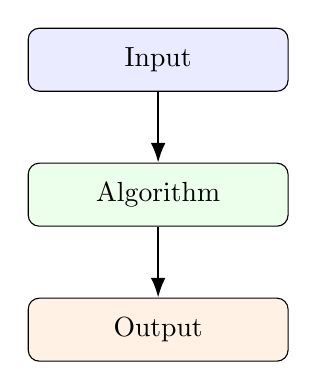
\begin{tikzpicture}[node distance=0.9cm]
        \node[draw, rounded corners, fill=blue!8, minimum width=3.3cm, minimum height=0.8cm] (i) {Input};
        \node[draw, rounded corners, fill=green!8, minimum width=3.3cm, minimum height=0.8cm, below=of i] (a) {Algorithm};
        \node[draw, rounded corners, fill=orange!10, minimum width=3.3cm, minimum height=0.8cm, below=of a] (o) {Output};
        \draw[-{Latex[length=2.5mm]}, thick] (i) -- (a);
        \draw[-{Latex[length=2.5mm]}, thick] (a) -- (o);
      \end{tikzpicture}
  \end{columns}
\end{frame}

%------------------------------------------------
\begin{frame}{Why pseudocode?}
  \begin{columns}[T]
    \column{0.49\textwidth}
      \textbf{Pseudocode} describes logic without worrying about one programming language's syntax.
      \vspace{0.8em}
      \begin{itemize}
        \item Easier to discuss before coding.
        \item Focuses on decisions and repetition.
        \item Makes algorithms easier to compare.
      \end{itemize}
    \column{0.47\textwidth}
      \begin{block}{Rule of thumb}
        Pseudocode should be detailed enough that a classmate can implement it without guessing the main idea.
      \end{block}
      \vspace{0.5em}
      \begin{alertblock}{Not the goal}
        Perfect syntax is less important than precise logic.
      \end{alertblock}
  \end{columns}
\end{frame}

%------------------------------------------------
\begin{frame}[fragile]{Basic pseudocode building blocks}
\begin{lstlisting}[style=pseudo]
x <- 0                  // assignment

if score >= 70 then     // decision
    grade <- "pass"
else
    grade <- "fail"

for i <- 1 to n do      // counted repetition
    print(i)

while x < target do     // condition-based repetition
    x <- x + 1
\end{lstlisting}

\vspace{-0.4em}
\begin{itemize}
  \item Use indentation to show which lines belong together.
  \item Choose meaningful variable names.
  \item State inputs and outputs when the algorithm is not obvious.
\end{itemize}
\end{frame}

%------------------------------------------------
\begin{frame}[fragile]{Example 1: Linear search}
\begin{block}{Problem}
Given an array $A$ and a value $x$, return the position of $x$ if it appears. Otherwise return \texttt{NOT-FOUND}.
\end{block}

\begin{lstlisting}[style=pseudo]
Algorithm LinearSearch(A, x)
Input: array A[1..n], target value x
Output: index of x, or NOT-FOUND

for i <- 1 to n do
    if A[i] = x then
        return i
return NOT-FOUND
\end{lstlisting}
\end{frame}

%------------------------------------------------
\begin{frame}{Tracing linear search}
  Suppose $A = [12, 7, 25, 4, 19]$ and $x = 4$.

  \vspace{0.6em}
  \begin{center}
  \begin{tabular}{cccccc}
    \toprule
    Step & $i$ & $A[i]$ & Compare $A[i]=4$? & Result & Continue? \\
    \midrule
    1 & 1 & 12 & no & -- & yes \\
    2 & 2 & 7  & no & -- & yes \\
    3 & 3 & 25 & no & -- & yes \\
    4 & 4 & 4  & yes & return 4 & no \\
    \bottomrule
  \end{tabular}
  \end{center}

  \vspace{0.8em}
  \begin{block}{Trace idea}
  A trace records how variables change while the algorithm runs.
  \end{block}
\end{frame}

%------------------------------------------------
\begin{frame}[fragile]{Example 2: Binary search}
\begin{block}{Key requirement}
Binary search only works when the array is sorted.
\end{block}

\begin{lstlisting}[style=pseudo,basicstyle=\ttfamily\scriptsize]
Algorithm BinarySearch(A, x)
low <- 1
high <- n

while low <= high do
    mid <- floor((low + high) / 2)
    if A[mid] = x then
        return mid
    else if A[mid] < x then
        low <- mid + 1
    else
        high <- mid - 1
return NOT-FOUND
\end{lstlisting}
\end{frame}

%------------------------------------------------
\begin{frame}{Binary search intuition}
  \begin{center}
    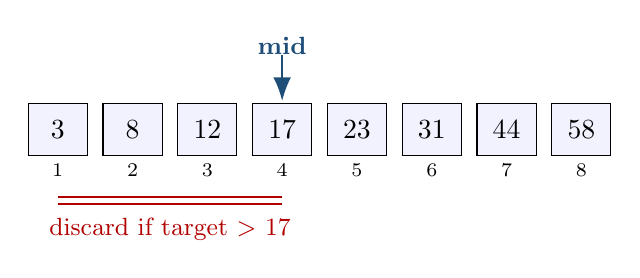
\begin{tikzpicture}[x=0.95cm,y=0.95cm]
      \foreach \i/\v in {1/3,2/8,3/12,4/17,5/23,6/31,7/44,8/58} {
        \node[draw, minimum width=0.75cm, minimum height=0.65cm, fill=blue!5] (n\i) at (\i,0) {\v};
        \node[font=\scriptsize] at (\i,-0.55) {\i};
      }
      \node[above=0.5cm of n4, font=\small\bfseries, color=Accent] {mid};
      \draw[-{Latex[length=3mm]}, thick, Accent] (4,1) -- (4,0.38);
      \draw[thick, red!70!black] (1,-0.9) -- node[below=4pt, font=\small] {discard if target $>$ 17} (4,-0.9);
      \draw[thick, red!70!black] (1,-1.0) -- (4,-1.0);
    \end{tikzpicture}
  \end{center}

  \vspace{0.5em}
  Each comparison removes about half of the remaining candidates.

  \vspace{0.5em}
  \begin{center}
    Linear search: $n$ candidates $\rightarrow$ Binary search: $\log_2 n$ rounds
  \end{center}
\end{frame}

%------------------------------------------------
\begin{frame}[fragile]{Example 3: Insertion sort}
\begin{block}{Idea}
Build a sorted prefix one item at a time. Insert the next item into the correct place.
\end{block}

\begin{lstlisting}[style=pseudo]
Algorithm InsertionSort(A)
for j <- 2 to n do
    key <- A[j]
    i <- j - 1
    while i > 0 and A[i] > key do
        A[i + 1] <- A[i]
        i <- i - 1
    A[i + 1] <- key
return A
\end{lstlisting}
\end{frame}

%------------------------------------------------
\begin{frame}{Insertion sort invariant}
  \begin{block}{Loop invariant}
  At the start of each outer-loop iteration, the subarray $A[1..j-1]$ is already sorted.
  \end{block}

  \vspace{0.6em}
  \begin{center}
  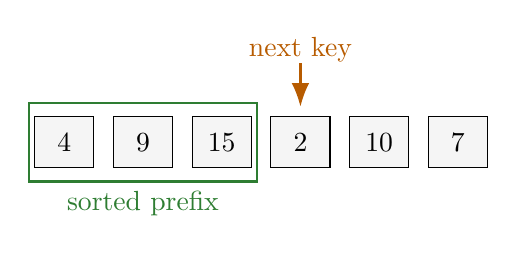
\begin{tikzpicture}
    \foreach \i/\v in {1/4,2/9,3/15,4/2,5/10,6/7} {
      \node[draw, minimum width=0.75cm, minimum height=0.65cm, fill=gray!8] (a\i) at (\i,0) {\v};
    }
    \draw[thick, Good] (0.55,-0.5) rectangle (3.45,0.5);
    \node[Good, below=0.5cm] at (2,0) {sorted prefix};
    \draw[-{Latex[length=3mm]}, thick, Warn] (4,1.0) -- (4,0.45);
    \node[Warn, above=.9cm] at (4,0) {next key};
  \end{tikzpicture}
  \end{center}

  \vspace{0.5em}
  Invariants help us explain why an algorithm is correct,\\not just how it runs.
\end{frame}

%------------------------------------------------
\begin{frame}{Running time: the basic question}
  \begin{columns}[T]
    \column{0.52\textwidth}
      Instead of timing on one computer, we ask:
      \begin{block}{As input size grows, how fast does the work grow?}
      Count the number of key operations as a function of $n$.
      \end{block}
      \begin{itemize}
        \item Linear search: at most $n$ comparisons.
        \item Binary search: about $\log_2 n$ comparisons.
        \item Insertion sort: up to about $n^2/2$ shifts/comparisons.
      \end{itemize}
    \column{0.43\textwidth}
      \begin{center}
      \begin{tabular}{cc}
        \toprule
        Name & Big-O \\
        \midrule
        Constant & $O(1)$ \\
        Logarithmic & $O(\log n)$ \\
        Linear & $O(n)$ \\
        Quadratic & $O(n^2)$ \\
        \bottomrule
      \end{tabular}
      \end{center}
  \end{columns}
\end{frame}

%------------------------------------------------
\begin{frame}{Correctness: what must be shown?}
  \begin{enumerate}
    \item \textbf{Preconditions}: What must be true before the algorithm starts?
    \item \textbf{Postconditions}: What must be true after it finishes?
    \item \textbf{Progress}: Why does each loop move toward stopping?
    \item \textbf{Invariant}: What useful fact stays true through each loop iteration?
  \end{enumerate}

  \vspace{0.6em}
  \begin{exampleblock}{Example}
  Binary search precondition: the input array is sorted. Without this, the algorithm may discard the wrong half.
  \end{exampleblock}
\end{frame}

%------------------------------------------------
\begin{frame}{Common pseudocode mistakes}
  \begin{columns}[T]
    \column{0.48\textwidth}
      \textbf{Avoid:}
      \begin{itemize}
        \item Using variables before defining them.
        \item Forgetting how indexes start: 0 or 1.
        \item Loops that never update the condition.
        \item Returning too early or too late.
      \end{itemize}
    \column{0.48\textwidth}
      \textbf{Prefer:}
      \begin{itemize}
        \item Clear input and output statements.
        \item Consistent indentation.
        \item Small examples to test edge cases.
        \item Comments for the main idea, not every line.
      \end{itemize}
  \end{columns}

  \vspace{0.7em}
  Edge cases to test: empty input, one element, duplicate values, missing target, already sorted data.
\end{frame}

%------------------------------------------------
\begin{frame}{Mini-assignment}
  Write pseudocode for this task:
  \begin{block}{Find the maximum value}
  Given a non-empty array $A[1..n]$, return the largest value in the array.
  \end{block}

  \vspace{0.5em}
  Then answer:
  \begin{enumerate}
    \item What variable stores the best value seen so far?
    \item How many comparisons are made?
    \item What happens when $n=1$?
  \end{enumerate}
\end{frame}

%------------------------------------------------
\begin{frame}[fragile]{One possible solution}
\begin{lstlisting}[style=pseudo]
Algorithm Maximum(A)
Input: non-empty array A[1..n]
Output: largest value in A

best <- A[1]
for i <- 2 to n do
    if A[i] > best then
        best <- A[i]
return best
\end{lstlisting}

\begin{block}{Running time}
The loop performs $n-1$ comparisons, so the algorithm is $O(n)$.
\end{block}
\end{frame}

%------------------------------------------------
\begin{frame}{Summary}
  \begin{itemize}
    \item Algorithms are precise recipes for transforming inputs into outputs.
    \item Pseudocode lets us focus on logic before programming syntax.
    \item Tracing helps catch mistakes and explain behavior.
    \item Big-O describes growth, not exact runtime on one machine.
    \item Correctness depends on assumptions, progress, and invariants.
  \end{itemize}

  \vspace{0.8em}
  \begin{center}
    \large Algorithm design = clarity + correctness + efficiency
  \end{center}
\end{frame}

%------------------------------------------------
%------------------------------------------------
\section{Part 2: Python and Jupyter}
%------------------------------------------------
%------------------------------------------------

%------------------------------------------------
\begin{frame}{Jupyter and IPython}

\href{https://jupyter.org}{Jupyter} provides an interactive environment for working with Python.

\begin{itemize}
  \item Execute code one cell at a time.
  \item Immediately inspect results.
  \item Combine code, text, equations, and visualizations.
  \item Experiment without repeatedly running an entire program.
  \item Use special \href{https://ipython.org}{IPython} ``magic'' commands.
\end{itemize}

\vspace{0.3cm}

Examples of magic commands:

\begin{center}
  \texttt{\%run \qquad \%timeit \qquad \%prun \qquad \%xmode}
\end{center}

\end{frame}

%------------------------------------------------
\begin{frame}[fragile]{Check and Install Python Packages}

Make sure a package is available before using it in Python.

\vspace{0.4em}

\textbf{In a terminal or command prompt:}

\begin{lstlisting}[language=bash]
# Show all installed packages
pip list

# Check one package
pip show pandas

# Install pandas if needed
pip install pandas
\end{lstlisting}

\vspace{0.3em}

\textbf{In Jupyter Notebook:}

\begin{lstlisting}[language=Python]
%pip install pandas
\end{lstlisting}

\vspace{0.3em}

If installation fails, check that Python and pip are using the same environment.

\end{frame}

%------------------------------------------------
\begin{frame}[fragile]{Load pandas and Read a CSV File}

\textbf{Goal:} Import pandas, load a CSV file, and preview the data.

\vspace{0.4em}

\begin{lstlisting}[language=Python]
# Load the pandas package
import pandas as pd

# Read a CSV file
df = pd.read_csv("data.csv")

# View the first five rows
df.head()
\end{lstlisting}

\vspace{0.4em}

\textbf{If the file is inside a folder:}

\begin{lstlisting}[language=Python]
df = pd.read_csv("data/myfile.csv")
\end{lstlisting}

\vspace{0.3em}

Replace \texttt{data.csv} with your own file name.

\end{frame}

%------------------------------------------------
\begin{frame}[fragile]{Python Functions}

A function packages reusable code into a named block.

\begin{lstlisting}[language=Python]
def square(x):
    return x ** 2

result = square(5)
print(result)
\end{lstlisting}

\textbf{Output:}

\begin{lstlisting}
25
\end{lstlisting}

Functions help make programs:

\begin{itemize}
  \item reusable,
  \item easier to understand,
  \item easier to test,
  \item easier to debug.
\end{itemize}

\end{frame}

%------------------------------------------------
\begin{frame}[fragile]{Functions with Multiple Inputs}

Functions can accept multiple arguments.

\begin{lstlisting}[language=Python]
def average(a, b):
    return (a + b) / 2

print(average(10, 20))
\end{lstlisting}

\textbf{Output:}

\begin{lstlisting}
15.0
\end{lstlisting}

\vspace{0.2cm}

A good function should generally perform one clearly defined task.

\end{frame}

%------------------------------------------------
\begin{frame}[fragile]{Why Functions Help}

\textbf{Without a function:}

\begin{lstlisting}[language=Python]
result1 = 5 ** 2
result2 = 8 ** 2
result3 = 12 ** 2
\end{lstlisting}

\textbf{With a function:}

\begin{lstlisting}[language=Python]
def square(x):
    return x ** 2

result1 = square(5)
result2 = square(8)
result3 = square(12)
\end{lstlisting}

The second version is easier to reuse and modify.

\end{frame}

%------------------------------------------------
\begin{frame}[fragile]{Running Python Files with \texttt{\%run}}

IPython allows Python scripts to be executed directly.

\begin{lstlisting}[language=Python]
%run my_script.py
\end{lstlisting}

If \texttt{my\_script.py} defines functions or variables, they can then
be available in the interactive IPython session.

\vspace{0.3cm}

This is useful when:

\begin{itemize}
  \item developing functions in separate Python files,
  \item testing scripts interactively,
  \item combining scripts with notebook analysis.
\end{itemize}

\end{frame}

%------------------------------------------------
\begin{frame}{What Is Debugging?}

Debugging is the process of finding and correcting errors in a program.

\vspace{0.3cm}

Common Python errors include:

\begin{itemize}
  \item \texttt{SyntaxError}
  \item \texttt{NameError}
  \item \texttt{TypeError}
  \item \texttt{IndexError}
  \item \texttt{KeyError}
  \item \texttt{ZeroDivisionError}
\end{itemize}

\vspace{0.3cm}

Python error messages provide information about where and why the program failed.

\end{frame}

%------------------------------------------------
\begin{frame}[fragile]{Example: A Bug}

Consider the following function:

\begin{lstlisting}[language=Python]
def divide(a, b):
    return a / b

divide(10, 0)
\end{lstlisting}

Python produces a traceback ending with:

\begin{lstlisting}
ZeroDivisionError: division by zero
\end{lstlisting}

The traceback tells us:

\begin{enumerate}
  \item what type of error occurred,
  \item where it occurred,
  \item which function calls led to it.
\end{enumerate}

\end{frame}

%------------------------------------------------
\begin{frame}{Reading a Traceback}

A useful strategy is to read a traceback from the bottom upward.

\begin{enumerate}
  \item Identify the exception type.
  \item Read the error message.
  \item Find the line where the error occurred.
  \item Follow the function-call chain if necessary.
  \item Inspect the values involved.
\end{enumerate}

\vspace{0.3cm}

The final line often provides the most important clue.

\end{frame}

%------------------------------------------------
\begin{frame}[fragile]{IPython Traceback Modes}

IPython provides the \texttt{\%xmode} magic command.

\begin{lstlisting}[language=Python]
%xmode Plain
%xmode Context
%xmode Verbose
\end{lstlisting}

The modes control how much information appears when an exception occurs.

\begin{itemize}
  \item \textbf{Plain}: minimal traceback.
  \item \textbf{Context}: includes surrounding context.
  \item \textbf{Verbose}: displays additional variable information.
\end{itemize}

\end{frame}

%------------------------------------------------
\begin{frame}[fragile]{Interactive Debugging}

IPython also supports interactive debugging.

After an exception:

\begin{lstlisting}[language=Python]
%debug
\end{lstlisting}

This allows you to inspect the program state near the point of failure.

Useful debugger commands can include:

\begin{itemize}
  \item inspecting variable values,
  \item moving through the call stack,
  \item identifying which inputs caused the error.
\end{itemize}

\end{frame}

%------------------------------------------------
\begin{frame}[fragile]{Debugger Commands}

\texttt{ipdb>} is the debugger prompt.

At that prompt, you can use commands such as:

\begin{lstlisting}
n       # next line
s       # step into function
c       # continue execution
p x     # print x
pp x    # pretty-print x
u       # move up one stack frame
d       # move down one stack frame
q       # quit debugger
\end{lstlisting}

\end{frame}

%------------------------------------------------
\begin{frame}{What Is Profiling?}

A program may be correct but still be slow.

\vspace{0.3cm}

\textbf{Profiling} means measuring where a program spends its time or memory.

\vspace{0.3cm}

The goal is to answer questions such as:

\begin{itemize}
  \item Which function is slow?
  \item Which line takes the most time?
  \item Which operation uses the most memory?
  \item Where should optimization effort be focused?
\end{itemize}

\vspace{0.3cm}

\textbf{Measure first; optimize second.}

\end{frame}

%------------------------------------------------
\begin{frame}[fragile]{Timing with \texttt{\%time}}

The \texttt{\%time} magic measures one execution.

\begin{lstlisting}[language=Python]
%time sum(range(1000000))
\end{lstlisting}

It reports information such as:

\begin{itemize}
  \item CPU time,
  \item system time,
  \item total execution time.
\end{itemize}

\vspace{0.3cm}

It is useful for obtaining a quick timing estimate.

\end{frame}

%------------------------------------------------
\begin{frame}[fragile]{Timing with \texttt{\%timeit}}

For more reliable measurements, use:

\begin{lstlisting}[language=Python]
%timeit sum(range(1000000))
\end{lstlisting}

\texttt{\%timeit} runs the statement repeatedly.

\vspace{0.3cm}

Advantages:

\begin{itemize}
  \item reduces the effect of random timing variation,
  \item automatically chooses an appropriate number of repetitions,
  \item makes it easier to compare different approaches.
\end{itemize}

\end{frame}

%------------------------------------------------
\begin{frame}[fragile]{Line Magic vs. Cell Magic}

A single percent sign applies to one line:

\begin{lstlisting}[language=Python]
%timeit sum(range(1000))
\end{lstlisting}

Two percent signs apply to an entire cell:

\begin{lstlisting}[language=Python]
%%timeit

total = 0
for i in range(1000):
    total += i
\end{lstlisting}

\end{frame}

%------------------------------------------------
\begin{frame}[fragile]{Function Profiling with \texttt{\%prun}}

Suppose we have:

\begin{lstlisting}[language=Python]
def calculate():
    total = 0
    for i in range(100000):
        total += i ** 2
    return total
\end{lstlisting}

Profile it with:

\begin{lstlisting}[language=Python]
%prun calculate()
\end{lstlisting}

\texttt{\%prun} reports which function calls consume the most time.

\end{frame}

%------------------------------------------------
\begin{frame}{More Profiling Tools}

The Python Data Science Handbook also introduces more detailed profiling tools.

\begin{description}
  \item[\texttt{\%lprun}] Line-by-line execution profiling.
  \item[\texttt{\%memit}] Memory usage of a statement.
  \item[\texttt{\%mprun}] Line-by-line memory profiling.
\end{description}

\vspace{0.4cm}

These tools can help identify a specific line of code responsible for poor performance.

\end{frame}

%------------------------------------------------
\begin{frame}{Recommended Workflow}

A practical Jupyter development workflow:

\begin{enumerate}
  \item Write a small function.
  \item Run and test the function.
  \item Inspect any traceback.
  \item Debug the problem.
  \item Confirm that the function is correct.
  \item Measure its performance.
  \item Profile slow sections.
  \item Optimize only the important bottlenecks.
\end{enumerate}

\end{frame}

%------------------------------------------------
\begin{frame}{Takeaways}

\begin{itemize}
  \item Functions organize Python code into reusable components.
  \item Jupyter makes experimentation and testing interactive.
  \item Tracebacks provide useful debugging information.
  \item IPython provides debugging tools such as \texttt{\%xmode} and \texttt{\%debug}.
  \item \texttt{\%time} and \texttt{\%timeit} measure execution time.
  \item Profiling reveals where optimization will have the greatest impact.
\end{itemize}

\end{frame}

%------------------------------------------------
\begin{frame}{Reference}


\includegraphics[height=3cm]{PDSH-cover.png}

Jake VanderPlas, \textbf{Python Data Science Handbook}

\tiny
\url{https://jakevdp.github.io/PythonDataScienceHandbook/01.00-ipython-beyond-normal-python.html}

\end{frame}

%------------------------------------------------
\begin{frame}{Assignment 1}

Submit your Jupyter Notebook on Canvas!

\begin{itemize}
\item \href{https://canvas.tamu.edu/courses/475969/assignments/3208733}{Assignment 1 on Cavnas}
\item \href{https://abuabara.github.io/DAEN300F26/events.csv}{Data: events.csv}
\end{itemize}
\end{frame}

\end{document}